\subsection{Measured outcomes}
All three terminal checkpoints are included. Table~\ref{tab:train04competence} separates denoiser competence from the two-call policy comparison. Table~\ref{tab:train04samplers} reports equal-seed descriptive means; full seed-specific results and source hashes are retained in the accompanying receipts.
\begin{table}[htbp]
\centering\small
\setlength{\tabcolsep}{4pt}
\caption{Held-out competence and sampling, by training seed. Accuracy and validity are percentages; marginal KL is in nats per masked bit. The denoiser calibration panel is separate from the sampling conditions.}
\label{tab:train04competence}
\begin{tabular}{@{}rlrrrrr@{}}
\toprule
Seed & Family & Det. acc. & Marg. KL & Info valid & Random valid & One valid\\
\midrule
17 & Systematic & 47.62 & 0.360 & 6.45 & 7.42 & 5.47\\
17 & Pair parity & 50.32 & 0.201 & 6.45 & 3.52 & 5.66\\
29 & Systematic & 52.38 & 0.350 & 7.62 & 9.18 & 6.45\\
29 & Pair parity & 49.68 & 0.197 & 7.62 & 5.08 & 6.25\\
43 & Systematic & 47.62 & 0.358 & 6.25 & 7.62 & 5.66\\
43 & Pair parity & 50.32 & 0.200 & 6.45 & 3.91 & 6.05\\
\bottomrule
\end{tabular}
\end{table}
For systematic, the equal-seed information-set minus random-halves validity difference is -1.30 percentage points, with paired condition-bootstrap95\% interval $[-3.91,1.24]$. The interval conditions on the three fitted checkpoints.
For paired parity, the equal-seed information-set minus random-halves validity difference is 2.67 percentage points, with paired condition-bootstrap95\% interval $[0.39,5.01]$. The interval conditions on the three fitted checkpoints.
\begin{table}[htbp]
\centering\small
\caption{Equal-seed decoder means. Coverage is the fraction of the 16 valid vectors observed among 32 draws per condition. Collision is the fraction of distinct draw pairs with identical outputs. Joint KL uses only two audit conditions per family and is not estimated for Bernoulli policies.}
\label{tab:train04samplers}
\begin{tabular}{@{}llrrrrr@{}}
\toprule
Family & Policy & Valid (\%) & Coverage (\%) & Collision (\%) & NFE & Joint KL\\
\midrule
Systematic & One round & 5.86 & 10.94 & 0.48 & 1.00 & 2.823\\
Systematic & Info set (2) & 6.77 & 12.76 & 0.35 & 2.00 & 2.825\\
Systematic & Random halves (2) & 8.07 & 16.15 & 0.37 & 2.00 & 2.828\\
Systematic & Bernoulli (2) & 6.71 & 12.76 & 0.43 & 2.00 & ---\\
Systematic & Bernoulli (4) & 5.92 & 11.33 & 0.43 & 3.92 & ---\\
Systematic & Bernoulli (8) & 5.86 & 10.16 & 0.50 & 7.48 & ---\\
Systematic & Sequential (8) & 5.79 & 10.55 & 0.41 & 8.00 & 2.826\\
Pair parity & One round & 5.99 & 11.33 & 0.39 & 1.00 & 2.823\\
Pair parity & Info set (2) & 6.84 & 13.15 & 0.42 & 2.00 & 2.825\\
Pair parity & Random halves (2) & 4.17 & 8.20 & 0.48 & 2.00 & 2.825\\
Pair parity & Bernoulli (2) & 6.38 & 11.85 & 0.40 & 2.00 & ---\\
Pair parity & Bernoulli (4) & 5.92 & 11.20 & 0.50 & 3.90 & ---\\
Pair parity & Bernoulli (8) & 4.82 & 8.98 & 0.47 & 7.53 & ---\\
Pair parity & Sequential (8) & 5.47 & 9.51 & 0.50 & 8.00 & 2.826\\
\bottomrule
\end{tabular}
\end{table}
\begin{figure}[htbp]
\centering
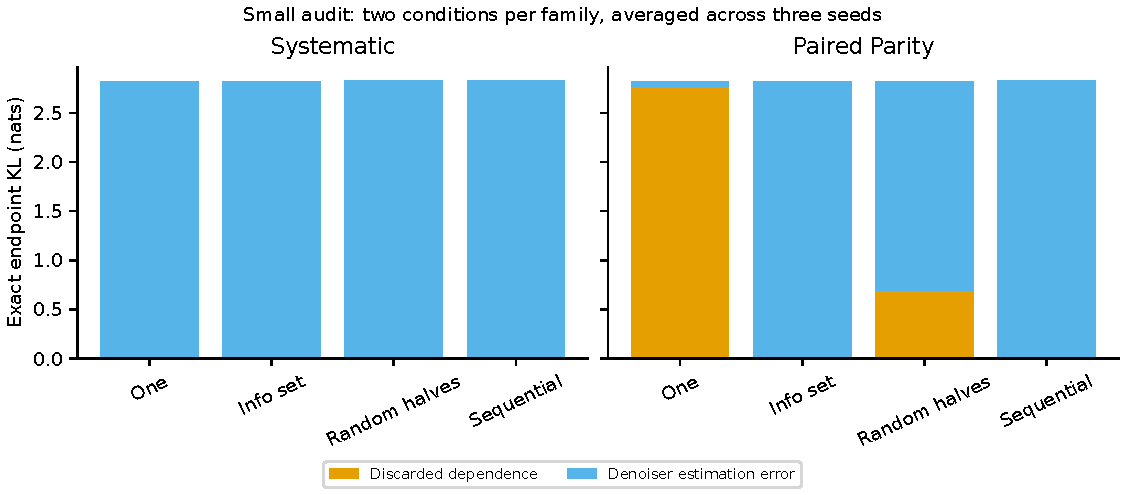
\includegraphics[width=\linewidth]{results/train04/final/figures/kl_decomposition.pdf}
\caption{Exact fixed-policy endpoint KL split into discarded dependence and denoiser estimation error on the small audit panel. The bars average the same two conditions per family across all three training seeds.}
\label{fig:train04decomposition}
\end{figure}
